\subsection{Thuật toán AES}
Vào năm 2000, Cơ quan quản lý về chuẩn và công nghệ của Mỹ, NIST (National Institute of Standard and Technology), đã tổ chức một cuộc thi để chọn một hệ mật mã mới thay thế cho DES. Hệ mã Rijndael đã đựợc chọn và được công bố (2002) như là chuẩn mật mã mới thay thế cho DES, với tên gọi là Advanced Encryption Standard (AES). Vào đến vòng trong còn có các ứng viên khác là RC6, Serpent, MARS và Twofish. Hệ mã này được phát triển bởi 2 nhà khoa học Bỉ, Joan Daemen và Vincent Rijnmen (vì vậy tên gọi Rijndael được tạo ra từ việc ghép tiền tố tên họ 2 ông này).\\
\indent AES được xây dựng trên nguyên lý thiết kế lưới giao hoán – thay thế (Substitution-Permutation Network). Đây là một hệ mã có tốc độ tốt trong cả cài đặt phần mềm cũng như phần cứng. Khác với DES, AES không theo mẫu thiết kế mạng Feistel. Thay vào đó các thao tác cơ bản được thực hiện trên các khối ma trận dữ liệu 4 $\times 4$ (bytes), được gọi là các trạng thái (state). Số vòng lặp của AES là một tham số xác định trên cơ sở kích thước khóa: 10 vòng lặp cho khóa 128 bit, 12 vòng cho 192 bit, 14 vòng cho 256 bit. Trong bài báo cáo này chúng em sẽ tìm hiểu sâu hơn về ASE-128.

\subsubsection{Quá trình mã hóa của Thuật toán AES-128}
Mã hóa AES được thực hiện thông qua 5 chức năng chính là AddRoundKey, SubBytes, ShiftRows, MixColumns và KeyExpansion. Năm chức năng này được sắp xếp để thực hiện ba bước cơ bản.
\begin{itemize}
    \item \textbf{Bước 1}: Bước khởi tạo: dữ liệu cần được mã hóa plain\_text[127:0] kết hợp với key[127:0] bằng chức năng AddRoundKey.
    \item \textbf{Bước 2}: Bước lặp mã hóa: kết quả bước 1 được sử dụng để thực hiện tuần tự các chức năng SubBytes, ShiftRows, MixColumns và AddRoundKey. Bước này được lặp lại 9 lần. Chú ý, KeyExpansion thực hiện song song với bước AddRoundKey để tạo khóa vòng cho chức năng này.
    \item \textbf{Bước 3}: Bước tạo ngõ ra: Sau 9 lần lặp ở bước 2, kết quả được sử dụng để thực hiện tuần tự các chức năng SubBytes, ShiftRows và AddRoundKey để tạo ngõ ra cipher\_text[127:0].
\end{itemize}
\begin{figure}[H]
    \centering
    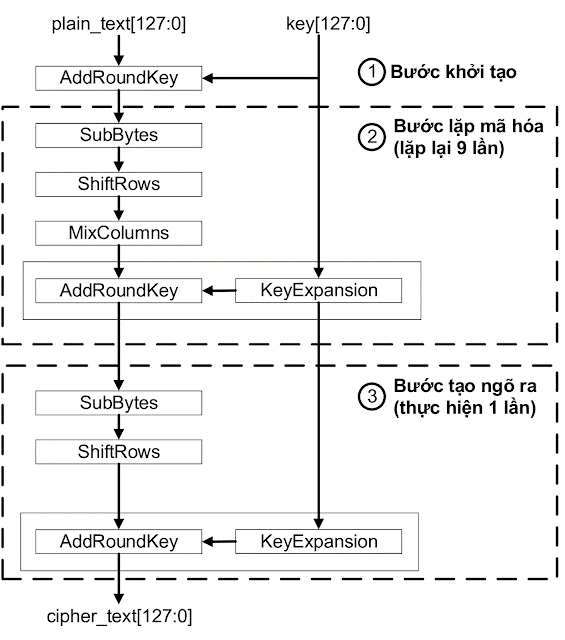
\includegraphics[width=\textwidth]{Ảnh/hiền/mã hóa aes.png}
    \caption{Quá trình mã hóa AES-128}
\end{figure}
Tất cả các phép toán được tổ hợp dựa vào phép tính XOR và các bảng dữ liệu nên rất nhanh và hiệu quả. Thuật toán cũng hiệu quả hơn cho các máy tính 32 bit.\\
VD: Giả sử chuỗi dữ liệu cần mã hóa plain\_text[127:0] và khóa mã key[127:0] có giá trị như sau:
\begin{itemize}
    \item plain\_text[127:0] = 32 43 f6 a8 88 5a 30 8d 31 31 98 a2 e0 37 07 34
    \item key[127:0] = 2b 7e 15 16 28 ae d2 a6 ab f7 15 88 09 cf 4f 3c
\end{itemize}
Dữ liệu và khóa mã được sắp xếp dưới dạng ma trận với mỗi phần tử là một byte.
\begin{figure}[H]
    \centering
    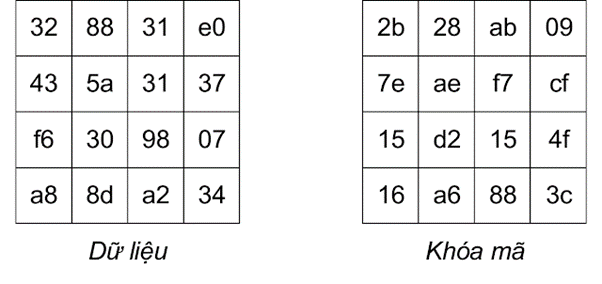
\includegraphics{Ảnh/hiền/vd aes.png}
    \caption{Dữ liệu và khóa mã được sắp xếp dưới dạng ma trận}
\end{figure}
Trong quá trình mã hóa, ma trận dữ liệu ban đầu sẽ bị biến đổi bởi các chức năng AddRoundKey, SubBytes, ShiftRows hoặc MixColumns để tạo ra các dữ liệu trung gian gọi là ma trận trạng thái. Ma trận khóa mã sẽ bị biến đổi bởi chức năng KeyExpansion để tạo ra các khóa mã trung gian gọi là khóa vòng.
\begin{itemize}
    \item \textbf{Chức năng AddRoundKey}: Chức năng AddRoundKey thực hiện ở:
    \begin{enumerate}
        \item Bước khởi tạo: $XOR$ khóa mã với ma trận dữ liệu
        \item Bước lặp mã hóa và bước tạo ngõ ra: $XOR$ khóa vòng (round key) với ma trận trạng thái. 
        \begin{figure}[H]
            \centering
            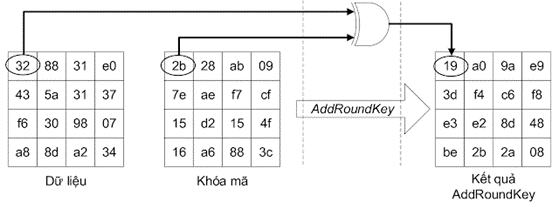
\includegraphics{Ảnh/hiền/addround.png}
            \caption{Chức năng AddRoundKey cho bước khởi tạo}
        \end{figure}
        Đối với bước lặp mã hóa và bước tạo ngõ ra, vị trí "khóa mã" là các "khóa vòng" còn dữ liệu là của lần tính trước đó.
    \end{enumerate}
    \item \textbf{Chức năng SubBytes}: Chức năng SubBytes là thực hiện thay thế từng byte của ma trận trạng thái, ngõ ra của AddRoundKey, bằng một giá trị đã quy định trong chuẩn AES. Bảng quy định giá trị thay thế gọi là S-box.
    \begin{figure}[H]
        \centering
        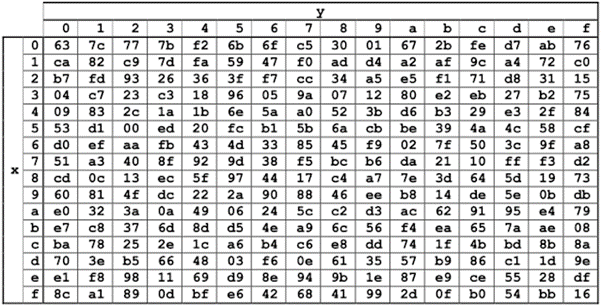
\includegraphics{Ảnh/hiền/s-box aes.png}
        \caption{S-box của mã hóa AES}
    \end{figure}
    Ví dụ, byte cần thay thế là H08 thì dò ở hàng số 0 và cột số 8 trong bảng S-box sẽ được kết quả là 30.
    \begin{figure}[H]
        \centering
        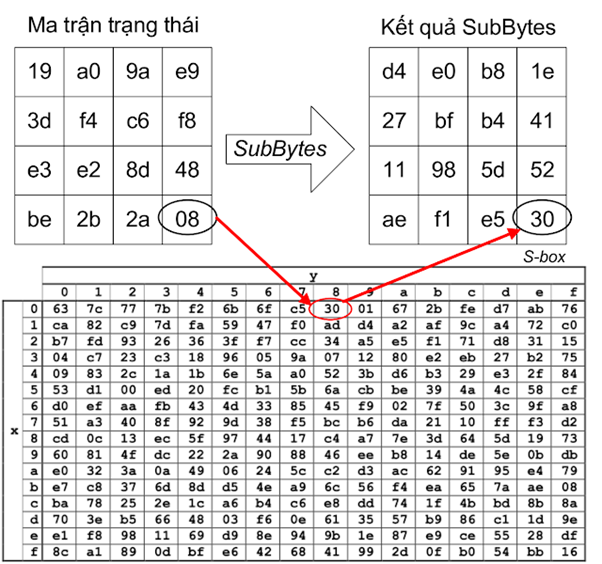
\includegraphics{Ảnh/hiền/vd h08.png}
        \caption{Mô tả kết quả biến đổi của H08}
    \end{figure}
    \item \textbf{Chức năng ShiftRows}: Chức năng ShiftRows thực hiện quay trái từng hàng của ma trận trạng thái, ngõ ra của SubBytes, theo byte với hệ số quay tăng dần từ 0 đến 3. Hàng đầu tiên có hệ số quay là 0 thì các byte được giữ nguyên vị trí. Hàng thứ hai có hệ số quay là 1 thì các byte được quay một byte. Hàng thứ ba quay hai byte và hàng thứ tư quay ba byte.
    \begin{figure}[H]
        \centering
        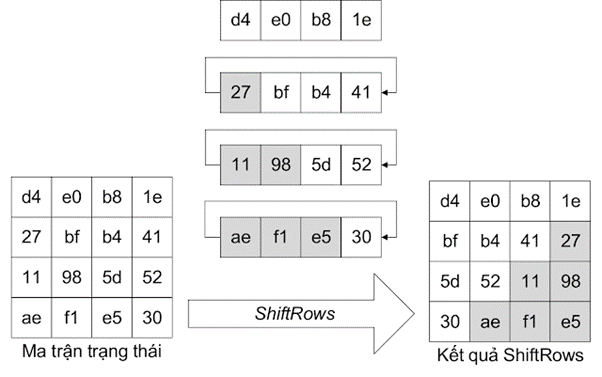
\includegraphics{Ảnh/hiền/shiftrow vd.png}
        \caption{Mô tả chức năng ShiftRows}
    \end{figure}
    \item \textbf{Chức năng MixColumns}: Chức năng MixColumns thực hiện nhân từng cột của ma trận trạng thái, ngõ ra của ShiftRows, với một ma trận chuyển đổi quy định bởi chuẩn AES.
    \begin{figure}[H]
        \centering
        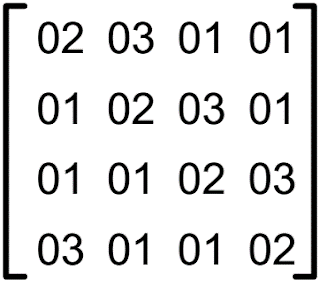
\includegraphics{Ảnh/hiền/mix.png}
        \caption{Ma trận chuyển đổi sử dụng trong chức năng MixColumns}
    \end{figure}
    Việc biến đổi một cột của ma trận trạng thái được thực hiện bởi hai phép toán là nhân và $XOR$.\\
    VD: Biểu thức sau tạo ra phần tử H04, H là ký hiệu của số Hex, ở cột 1 trong hình minh họa "chức năng MixColumns".\\
    $H04 =Hd4.H02 + Hbf.H03 + H5d.H01 + H30.H01=Hd4.H02 + (Hbf.H02 + Hbf.H01) + H5d.H01 + H30.H01$ 
    \begin{figure}[H]
        \centering
        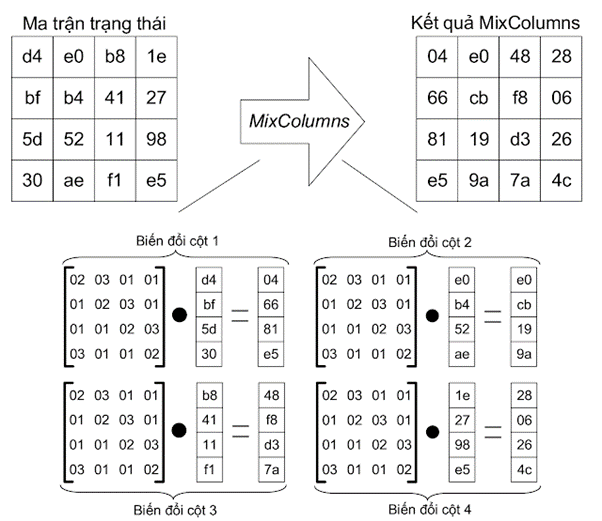
\includegraphics{Ảnh/hiền/vd mix.png}
        \caption{Mô tả chức năng MixColoumns}
    \end{figure}
    Phép nhân với H01 thì giữ nguyên giá trị. Phép nhân với H02 tương đương với việc dịch trái một bit và XOR có điều kiện như sau:
    \begin{itemize}
        \item Nếu bit MSB của giá trị được dịch bằng 1 thì giá trị sau khi dịch được $XOR$ với H1b.
        \item Nếu bit MSB của giá trị được dịch bằng 0 thì giữ giá trị sau khi dịch.
    \end{itemize}
    \begin{figure}[H]
        \centering
        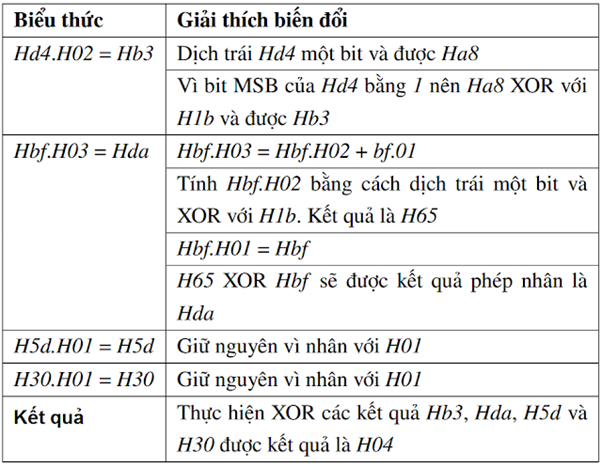
\includegraphics{Ảnh/hiền/mix h04.png}
        \caption{Chi tiết về cách tính MixColoums tạo ra phần từ H04 ở cột 1}
    \end{figure}
    \item \textbf{Chức năng KeyExpansion}: \\
    Chức năng KeyExpansion thực hiện tính toán khóa vòng cho bước lặp mã hóa và bước tạo ngõ ra. Kết quả của một lần thực thi KeyExpansion là một khóa vòng sử dụng cho chức năng AddRoundKey. Với mã hóa AES-128, số khóa vòng là 10 tương ứng với 9 lần AddRoundKey ở bước lặp mã hóa và 1 lần AddRoundKey ở bước tạo ngõ ra.\\
    Chức năng KeyExpansion được thực hiện thông qua 4 chức năng là RotWord, SubWord, AddRcon và AddW.
    \begin{figure}[H]
        \centering
        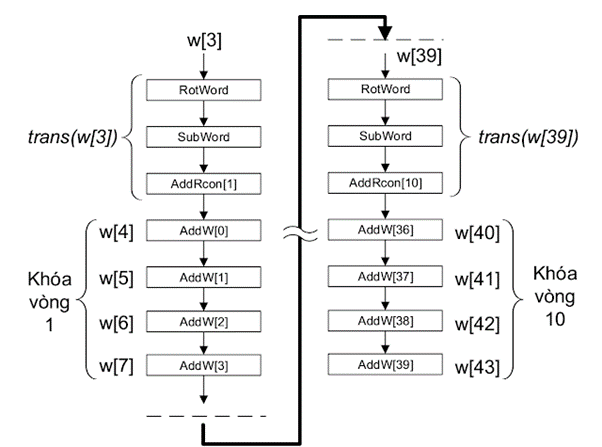
\includegraphics{Ảnh/hiền/keyexpan.png}
        \caption{Chức năng KeyExpansion}
        
    \end{figure}
    Mỗi khóa vòng có 128 bit được chia làm 4 word, mỗi word là 4 byte và ký hiệu là w[j] với j là số nguyên. Mã hóa AES-128 có 1 khóa mã và 10 khóa vòng nên tổng số từ là 44 và được đánh số từ 0 đến 43. Khóa mã có 4 từ là w[0], w[1], w[2] và w[3]. Khóa vòng 1 có 4 từ là w[4], w[5], w[6] và w[7]. Tương tự, khóa vòng 10 có 4 từ là w[40], w[41], w[42] và w[43].\\
    Từ w[j] tính theo công thức sau, với 3 < j < 44.\\
    $w[j] = AddW[j - 4] = w[j - 1] + w[j - 4]$ \\  
    $w[j = 4*n] = AddW[j - 4] = trans(w[j - 1])+ w[j - 4]$\\
    Chú ý, khi tính các từ ở vị trí j là bội số của 4, như w[4], w[8],... và w[40], thì w[j-1] phải được biến đổi qua 3 chức năng RotWord, SubWord và AddRcon, gọi là trans(w[j-1]), trước khi XOR với w[j-4].\\
    Khóa mã key ở mục 1 được sử dụng để minh họa việc tính toán khóa vòng. Khóa mã key[127:0] được chia làm 4 từ như biểu thức sau:\\
    $w[0] = 2b7e1516 w[1] = 28aed2a6$ \\
    $w[2] = abf71588 w[3] = 09cf4f3c$\\
    Việc tính toán khóa vòng 1 là thực hiện tính 4 từ w[4], w[5], w[6] và w[7]. Để tính khóa vòng 1, trans(w[3]) phải được tính trước thông qua 3 chức năng RotWord, SubWord và AddRcon.\\
    $w[4] = AddW[0] = trans(w[3])+ w[0]w[5] = AddW[1] = w[4]+ w[1]w[6] = AddW[2] = w[5]+ w[2]w[7] = AddW[3] = w[6]+ w[3]$\\
    Chức năng RotWord Chức năng RotWord thực hiện quay trái từ w[j] một byte.
    \begin{figure}[H]
        \centering
        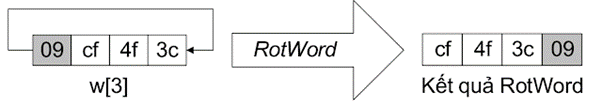
\includegraphics{Ảnh/hiền/rword.png}
        \caption{Thực thi RotWord cho từ w[3]}
    \end{figure}
    Chức năng SubWord thực hiện thay thế các phi tuyến từng byte của kết quả RotWord theo bảng S-box.
    \begin{figure}[H]
        \centering
        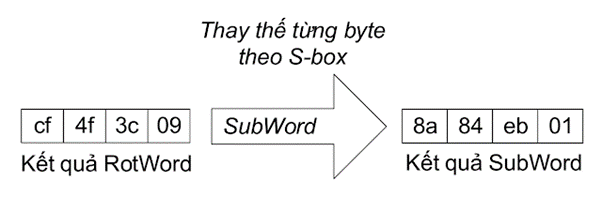
\includegraphics{Ảnh/hiền/subw.png}
        \caption{Thực thi SubWord khi chuyển đổi từ w[3]}
    \end{figure}
    Chức năng AddRcon thực hiện XOR kết quả SubWord và giá trị Rcon[j/4] với j là bội số của 4. Số lượng giá trị Rcon[j/4] là 10 tương ứng với 10 lần tính khóa vòng. Chức năng AddRcon sẽ tạo ra kết quả cuối cùng của biến đổi trans(w[j-1]).
    \begin{tabular}{|c|c|c|}
    
\hline
\textbf{Rcon[j/4]} & \textbf{Giá trị HEX} & \textbf{Vị trí sử dụng} \\
\hline
Rcon[1] & 01000000 & sử dụng cho trans(w[3]) khi tính w[4] \\
Rcon[2] & 02000000 & sử dụng cho trans(w[7]) khi tính w[8] \\
Rcon[3] & 04000000 & sử dụng cho trans(w[11]) khi tính w[12] \\
Rcon[4] & 08000000 & sử dụng cho trans(w[15]) khi tính w[16] \\
Rcon[5] & 10000000 & sử dụng cho trans(w[19]) khi tính w[20] \\
Rcon[6] & 20000000 & sử dụng cho trans(w[23]) khi tính w[24] \\
Rcon[7] & 40000000 & sử dụng cho trans(w[27]) khi tính w[28] \\
Rcon[8] & 82000000 & sử dụng cho trans(w[31]) khi tính w[32] \\
Rcon[9] & 1b000000 & sử dụng cho trans(w[35]) khi tính w[36] \\
Rcon[10] & 36000000 & sử dụng cho trans(w[39]) khi tính w[40] \\
\hline
\end{tabular}
\begin{figure}[H]
    \centering
    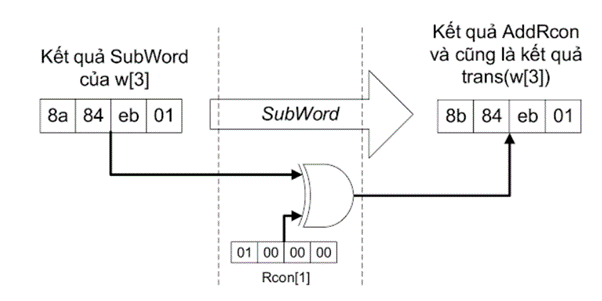
\includegraphics{Ảnh/hiền/addcon.png}
    \caption{Thực thi AddRcon khi chuyển đổi từ w[3]}
\end{figure}
Chức năng AddW thực hiện XOR w[j-4] với w[j-1] hoặc trans(w[j-1]) như công thức 4.8 để tạo ra khóa vòng.
\begin{figure}[H]
    \centering
    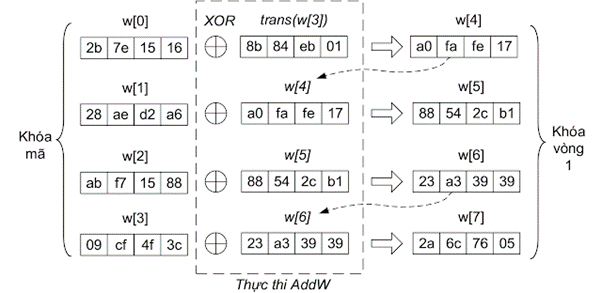
\includegraphics{Ảnh/hiền/addw.png}
    \caption{Thực thi AddW}
\end{figure}
\end{itemize}
\subsubsection{Quá trình giải mã của Thuật toán AES-128}

Mã hóa chuyển một "bản rõ" (Plaintext) thành một "bản mã" (Ciphertext) thông qua một khóa mã (key) giúp che dấu thông tin gốc ban đầu. Giải mã là quá trình nghịch đảo (Inverse Cipher) của quá trình mã hóa. Nó giúp khôi phục lại bản rõ từ một bản mã \cite{abdullah2017advanced}.

Thuật toán giải mã khá giống với thuật toán mã hóa về mặt cấu trúc nhưng 4 hàm sử dụng là 4 hàm ngược của quá trình mã hóa.
\begin{figure}[H]
    \centering
    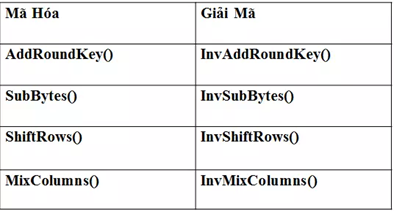
\includegraphics[scale=1]{pic/huê/ngc mã hóa.png}
    
    
    \caption{Các chức năng ngược nhau trong mã hóa và giải mã AES}
\end{figure}

Các bước giải mã:
\begin{itemize}
    \item Bước 1. Bước khởi tạo: Dữ liệu cần được mã hóa cipher\_text[127:0] kết hợp với khóa vòng thứ 10, round\_key\_10[127:0], bằng chức năng AddRoundKey.
    \item Bước 2. Bước lặp giải mã: kết quả bước 1 được sử dụng để thực hiện tuần tự các chức năng InvShiftRows, InvSubBytes, AddRoundKey và InvMixColumns. Bước này được lặp lại 9 lần.
    \item Bước 3. Bước tạo ngõ ra: Sau 9 lần lặp ở bước 2, kết quả được sử dụng để thực hiện tuần tự các chức năng InvShiftRows, InvSubBytes và AddRoundKey với khóa mã ban đầu để khôi phục lại plain\_text[127:0].
\end{itemize}

So sánh giữa quá trình mã hóa và giải mã như sau:

\begin{figure}[H]
    \centering
    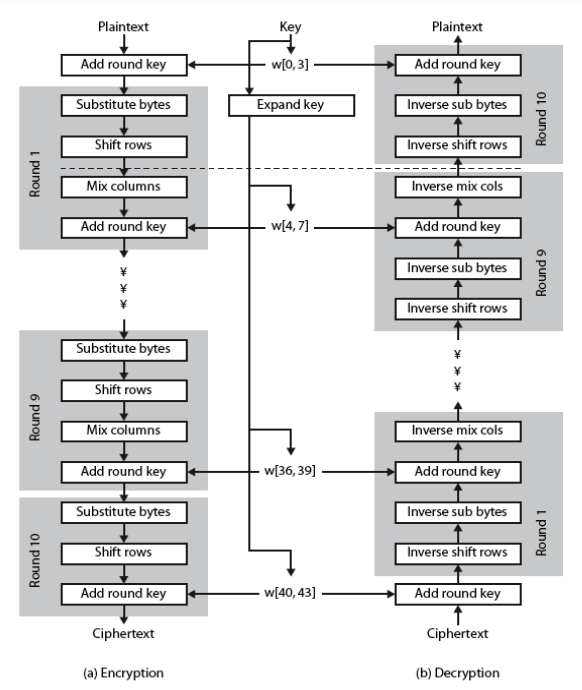
\includegraphics[scale=1.4]{pic/huê/AES mã hóa và giải mã.png}
    
    
    \caption{Quá trình mã hóa và giải mã AES}
\end{figure}

Quá trình giải mã AES-128 sẽ được giải thích trên một ví dụ cụ thể. Giả sử chuỗi dữ liệu cần mã hóa cipher\_text[127:0] và khóa vòng cuối cùng lấy từ quá trình mã hóa key[127:0] có giá trị như sau:
\begin{itemize}
    \item cipher\_text[127:0] =  69 c4 e0 d8 6a 7b 04 30 d8 cd b7 80 70 b4 c5 5a.
    \item key[127:0] = 13 11 1d 7f e3 94 4a 17 f3 07 a7 8b 4d 2b 30 c5.
\end{itemize}

Dữ liệu và khóa mã được sắp xếp dưới dạng ma trận với mỗi phần tử là một byte.
\begin{figure}[H]
    \centering
    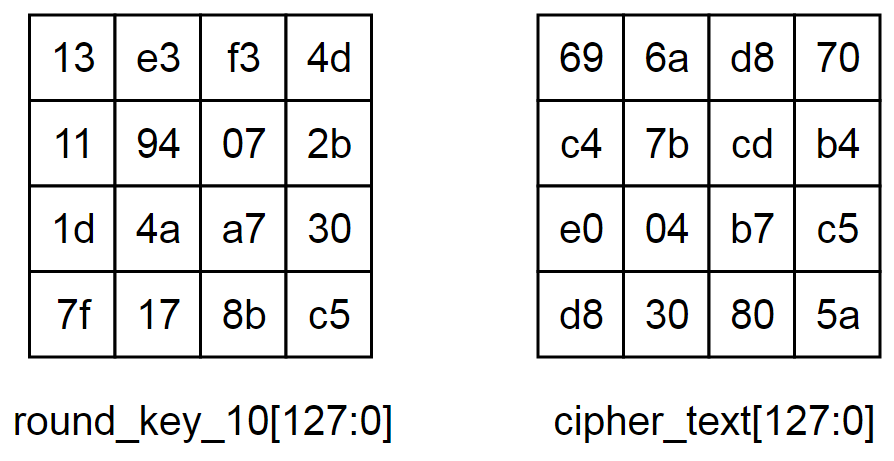
\includegraphics[scale=0.4]{pic/huê/input giải mã.png}
    
    
    \caption{Ma trận khóa vòng thứ 10 và ma trận dữ liệu đã mã hóa}
\end{figure}

\begin{itemize}
    \item Chức năng InvAddRoundKey:

    Chức năng InvAddRoundKey trong quá trình giải mã cũng chính là chức năng AddRoundKey trong quá trình mã hóa nên gọi chung là AddRoundKey.\cite{b3}

    \begin{figure}[H]
    \centering
    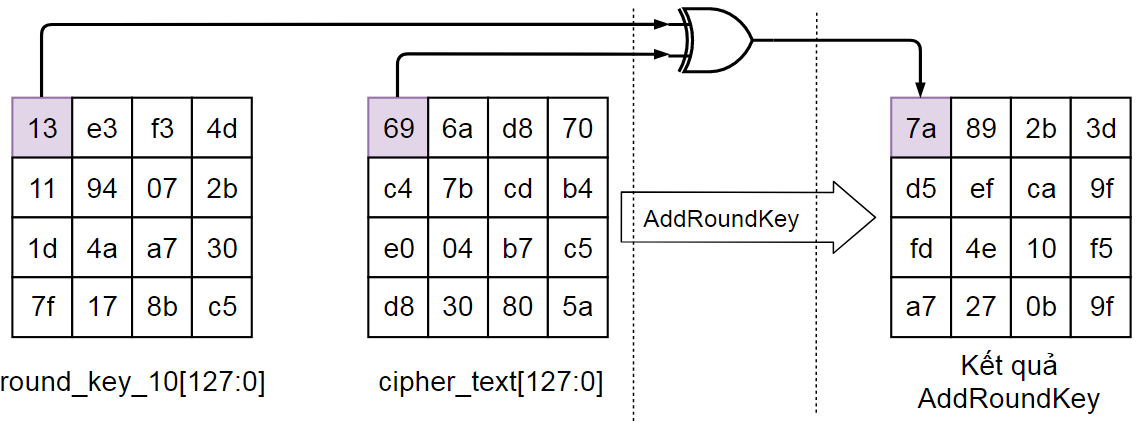
\includegraphics[scale=0.4]{pic/huê/Chức năng AddRoundKey đảo.png}
    
    
    \caption{Chức năng InvAddRoundKey}
\end{figure}
\item Chức năng InvShiftRows:
InvShiftRows là đảo của chức năng ShiftRows. InvShiftRows thực hiện quay phải từng hàng của ma trận trạng thái, sinh ra từ bước trước đó, theo byte với hệ số quay tăng dần từ 0 đến 3. Hàng đầu tiên có hệ số quay là 0 thì các byte được giữ nguyên vị trí. Hàng thứ hai có hệ số quay là 1 thì các được quay một byte. Hàng thứ ba quay hai byte và hàng thứ tư quay ba byte \cite{fips2001197}.
\begin{figure}[H]
    \centering
    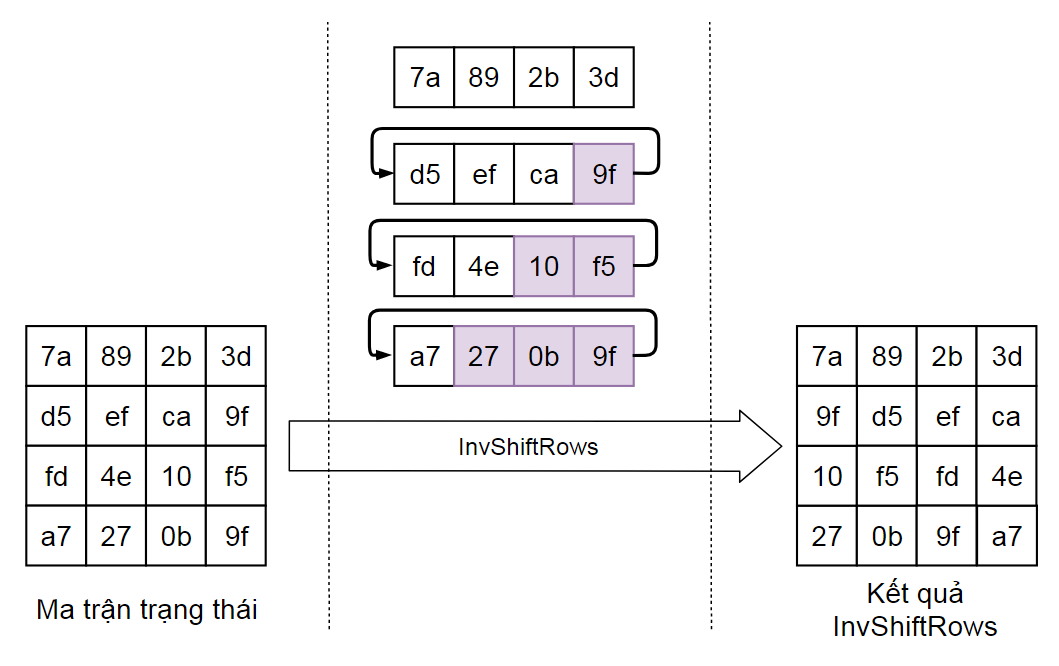
\includegraphics[scale=0.4]{pic/huê/Chức năng InvShiftRows.png}
    
    
    \caption{Chức năng InvShiftRows}
\end{figure}
\item Chức năng InvSubBytes:
Chức năng InvSubBytes là thực hiện thay thế từng byte của ma trận trạng thái, bằng một giá trị đã quy định trong chuẩn AES. Bảng quy định giá trị thay thế cho InvSubBytes gọi là S-box đảo (Inverse S-box) \cite{fips2001197}.
\begin{figure}[H]
    \centering
    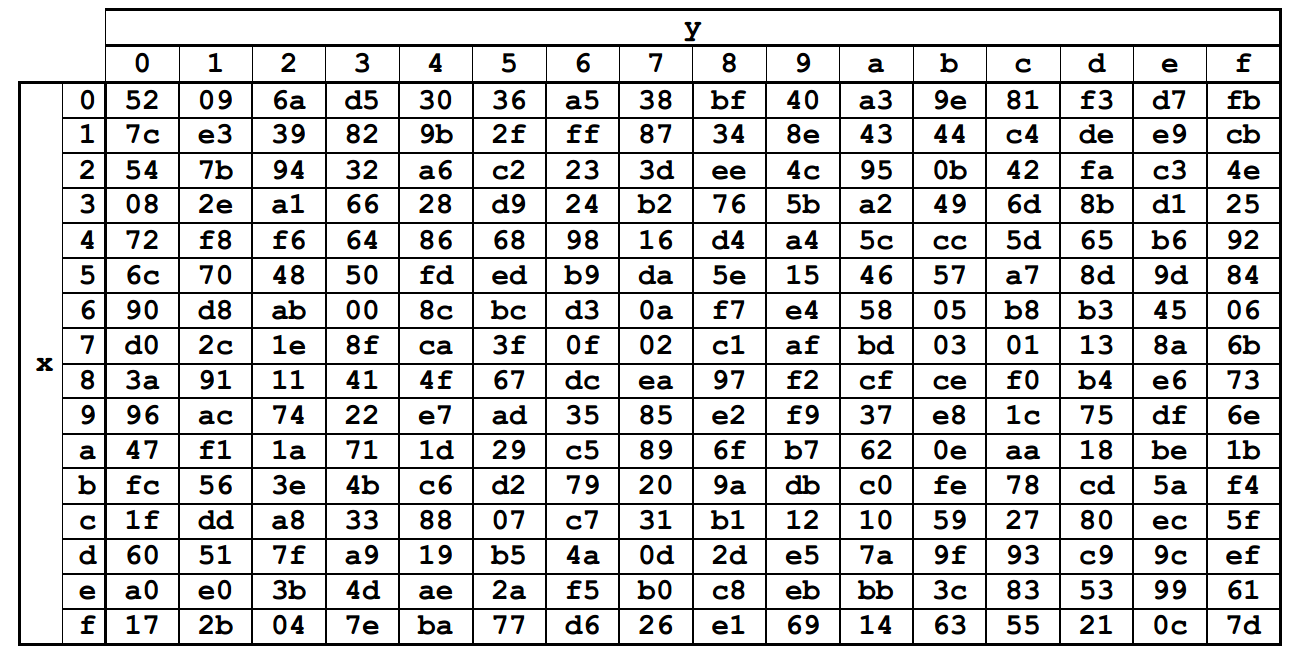
\includegraphics[scale=0.3]{pic/huê/bảng S-box Inv.png}
    
    \caption{Bảng S-box đảo của chuẩn AES}
\end{figure}
Ví dụ, byte cần thay thế là Ha7 thì dò ở hàng "a" và cột số 7 trong bảng S-box đảo sẽ được kết quả là H89.
\begin{figure}[H]
    \centering
    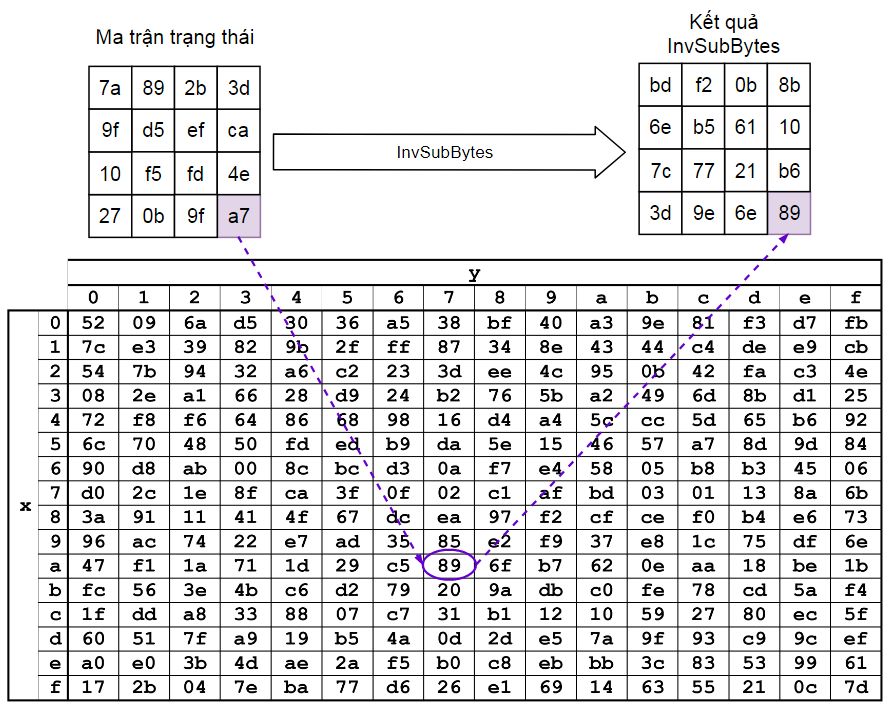
\includegraphics[scale=0.5]{pic/huê/Chức năng InvSubBytes.png}
    
    \caption{Chức năng InvSubBytes}
\end{figure}
\item Chức năng InvMixColumns:

InvMixColumns của quá trình giả mã là đảo của MixColumns trong quá trình mã hóa. Từng cột của ma trận trạng thái sẽ được nhân với ma trận chuyển đổi sau đây.\cite{fips2001197}

\begin{figure}[H]
    \centering
    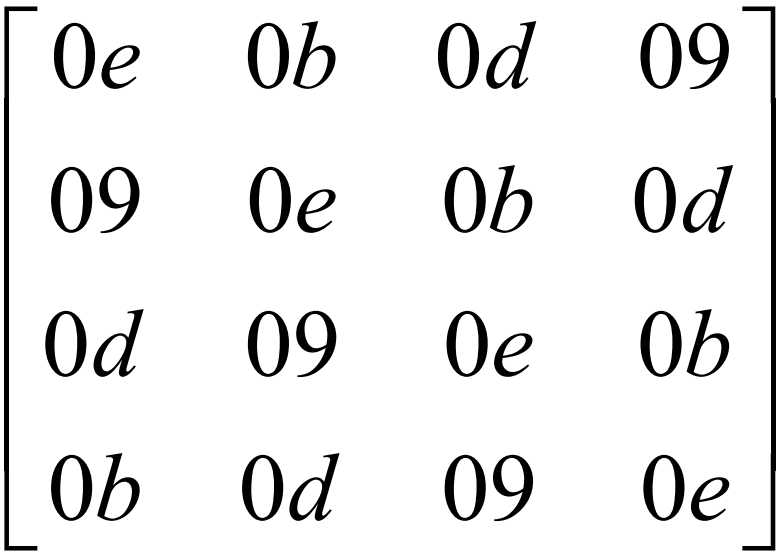
\includegraphics[scale=0.2]{pic/huê/Ma trận chuyển đổi dùng trong InvMixColumns.png}
    
    \caption{Ma trận chuyển đổi dùng trong InvMixColumns}
\end{figure}

Cách tính InvMixColumns sẽ được trình bày sau đây: \\

\textbf{Phép nhân một byte A với H0e:}
\begin{center}
    $A.H0e = A.H08 + A.H04 + A.H02$
\end{center}

    Trong đó, phép nhân với H04 và H08 hoàn toàn có thể chuyển về phép nhân với H02:
\begin{center}
    $A.H04 = A.H02.H02$
    
$A.H08 = A.H02.H02.H02 $
\end{center}
    
Suy ra: 
\begin{center}
    $A.H0e = A.H02.H02.H02 + A.H02.H02 + A.H02 $
\end{center}

\textbf{Phép nhân một byte A với H0b:}
\begin{center}
    $A.H0b = A.H08 + A.H02 + A.H01 = A.H02.H02.H02 + A.H02 + A.H01 $
\end{center}

\textbf{Phép nhân một byte A với H0d:}
\begin{center}
    $A.H0d = A.H08 + A.H04 + A.H01 = A.H02.H02.H02 + A.H02.H02 + A.H01 $
\end{center}

\textbf{Phép nhân một byte A với H09:}
\begin{center}
    $A.H0e = A.H08 + A.H01 = A.H02.H02.H02 + A.H01$
\end{center}

Việc tính InvMixColumn cho toàn bộ một ma trận trạng thái như sau:

\begin{figure}[H]
    \centering
    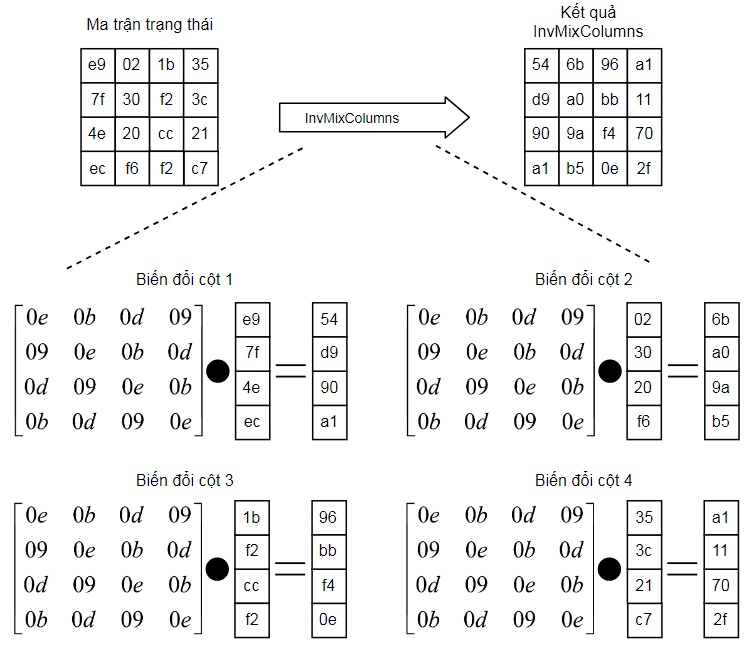
\includegraphics[scale=0.5]{pic/huê/Chức năng InvMixColumns.png}
    
    \caption{Chức năng InvMixColumns}
\end{figure}

Với việc quy đổi phép nhân về dạng nhân với H02 và H01. Mạch logic nhân một byte với H0e, H0b, H0d và H09 có thể được thực hiện như hình sau.

\begin{figure}[H]
    \centering
    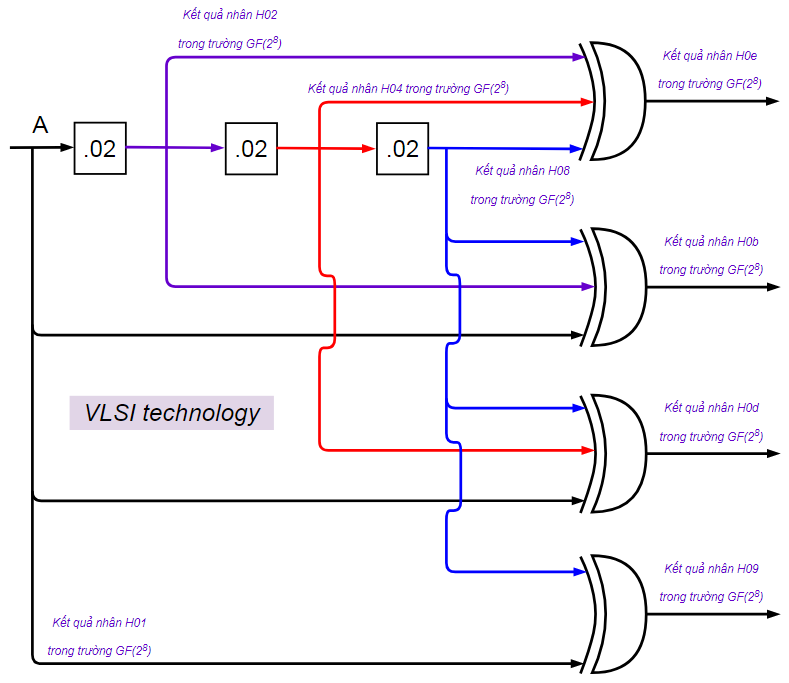
\includegraphics[scale=0.5]{pic/huê/Mạch nguyên lý nhân một byte A với các phần tử trong ma trận chuyển đổi InvMixColumns.png}
    
    \caption{Mạch nguyên lý nhân một byte A với các phần tử trong ma trận chuyển đổi InvMixColumns}
\end{figure}
\end{itemize}

\subsubsection{Các dạng tấn công vào AES}
\begin{itemize}
    \item Side-channel Attack:
    \begin{itemize}
        \item Side Channels (Kênh kề) được định nghĩa là các kênh đầu ra không mong muốn từ một hệ thống.
        \item Tấn công kênh bên hay còn gọi là Tấn công kênh kề là loại tấn công dễ thực hiện trong các loại tấn công mạnh chống lại quá trình triển khai mã hóa, và mục tiêu của loại tấn công này là phân tích các nguyên tố, các giao thức, module, và các thiết bị trong mỗi hệ thống.
        \item Một số loại tấn công kênh kề như: Tấn công thời gian, tấn công dựa vào lỗi, tấn công phân tích năng lượng, tấn công phân tích điện từ
        \item Tấn công kênh bên hay còn gọi là Tấn công kênh kề là loại tấn công dễ thực hiện trong các loại tấn công mạnh chống lại quá trình triển khai mã hóa, và mục tiêu của loại tấn công này là phân tích các nguyên tố, các giao thức, module, và các thiết bị trong mỗi hệ thống.
        \item Một số loại tấn công kênh kề như: Tấn công thời gian, tấn công dựa vào lỗi, tấn công phân tích năng lượng, tấn công phân tích điện từ.
    \end{itemize}

    \item Known Attacks:
    \begin{itemize}
        \item Vào năm 2002, Nicolas Courtois và Josef Pieprzyk phát hiện một tấn công trên lý thuyết gọi là tấn công XSL và chỉ ra điểm yếu tiềm tàng của AES.
        \item Tuy nhiên, một vài chuyên gia về mật mã học khác cũng chỉ ra một số vấn đề trong Cơ sở Toán học của tấn công này và cho rằng các tác giả đã có sai lầm trong tính toán. Việc tấn công dạng này có thực sự trở thành hiện thực hay không vẫn còn để ngỏ và cho tới nay thì tấn công XSL vẫn chỉ là suy đoán.
    \end{itemize}
\end{itemize}

\subsubsection{Mặt hạn chế của AES }
\begin{itemize}
    \item Phương pháp phát triển AES tập trung vào việc tăng số vòng hoặc kích thước khối thay vì tìm kiếm giải pháp tốt nhất.
    \item Quá trình giải mã bằng cấu trúc AES chậm hơn quá trình mã hóa, đặc biệt là trên các thiết bị nhúng, đồng nghĩa với sự mất cân bằng trong cấu trúc mã hóa và giải mã cho một số thiết bị.
    \item Quá trình mã hóa cho hàng nghìn bit sẽ tạo ra sự khác biệt rõ ràng về thời gian giữa mã hóa và giải mã do bộ tích lũy cho phép lặp lại hàng nghìn vòng, dẫn đến sự khác biệt rõ ràng.
    \item Thuật toán mã hóa AES hoạt động với 128 bit văn bản gốc hoặc 16 byte và tất cả các thao tác nội bộ dựa trên triển khai theo byte, có nghĩa là giá trị tối đa có thể được thực hiện theo thập lục phân là (FF).
    \item Thuật toán mã hóa AES 11 vòng có thể không đủ an toàn cho các ứng dụng xử lý dữ liệu lớn. Lý do là vì thuật toán này chỉ có 128 bit khóa, trong khi các ứng dụng dữ liệu lớn có thể cần nhiều bit khóa hơn để đảm bảo bảo mật. Ngoài ra, thuật toán AES 11 vòng có thể quá chậm cho các ứng dụng dữ liệu lớn.
    \item S-Box cố định với hai bảng 256 giá trị ở dạng ký hiệu lục phân có thể tạo thành một mục tiêu tốt cho các cuộc tấn công, vì mỗi giá trị có một ánh xạ đến giá trị tương ứng trong bảng.
    \item Các khóa có độ dài 128-bit, 192-bit và 256-bit. Nói chung, các khóa này được coi là có độ dài thực tế chỉ trong trường hợp của khóa 128-bit, còn lại hai khóa khác được coi là không có độ dài thực sự là 192-bit và 256-bit.
     Lý do chính cho việc xem xét các khóa 192-bit và 256-bit là không có độ dài thực tế là do quá trình XORing (phép toán XOR) giữa khóa và ma trận trạng thái không phù hợp với cùng một kích thước. Trong các vòng lặp sau của quá trình mã hóa AES, khóa ban đầu được mở rộng thành các khóa con khác (Key Schedule) để tạo ra các khóa con cho mỗi vòng. Tuy nhiên, do sự không phù hợp về kích thước, việc XORing khóa với ma trận trạng thái chỉ tăng khả năng của không gian tìm kiếm cho việc tạo ra khóa cho các vòng lặp còn lại mà không cung cấp sự tăng cường đáng kể về độ bảo mật.
    Do đó, mặc dù AES cho phép sử dụng các khóa có độ dài khác nhau, thực tế, việc sử dụng các khóa có độ dài lớn hơn 128-bit không đem lại sự cải thiện rõ rệt về mặt bảo mật, và trong một số trường hợp có thể chỉ tăng chi phí tính toán mà không cải thiện được mức độ bảo mật \cite{dawood2017analytical}.
\end{itemize}



